\documentclass{article}




\usepackage{tikz}
\usetikzlibrary{datavisualization}
\usetikzlibrary{datavisualization.formats.functions}
\begin{document}
\centerline{\sc \large A Simple Sample \LaTeX\ File}
\vspace{.5pc}
\centerline{\sc Stupid Stuff I Wish Someone Had Told Me Four Years Ago}
\centerline{\it (Read the .tex file along with this or it won't 
            make much sense)}

\begin {center}
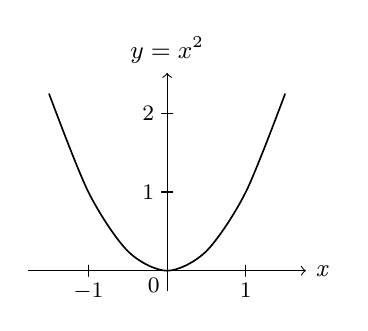
\begin{tikzpicture}
\datavisualization [school book axes,
                    visualize as smooth line,
                    y axis={label={$y=x^2$}},
                    x axis={label} ]

data [format=function] {
      var x : interval [-1.5:1.5] samples 7;
      func y = \value x*\value x;
      };
\end{tikzpicture}
\vspace{2pc}

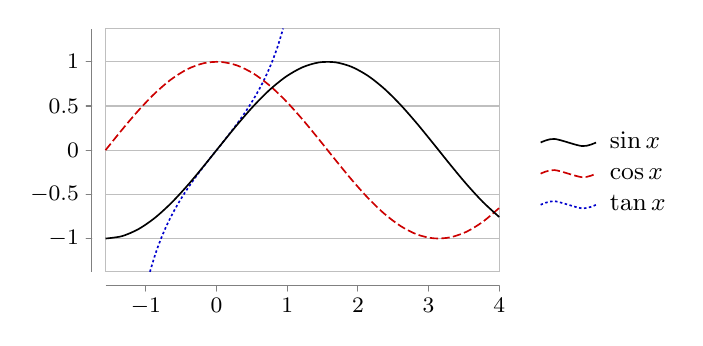
\begin{tikzpicture}
\datavisualization [scientific axes=clean,
                    y axis=grid,
                    visualize as smooth line/.list={sin,cos,tan},
                    style sheet=strong colors,
                    style sheet=vary dashing,
                    sin={label in legend={text=$\sin x$}},
                    cos={label in legend={text=$\cos x$}},
                    tan={label in legend={text=$\tan x$}},
                    data/format=function
                    ]
data [set=sin] {
  var x : interval [-0.5*pi:4];
  func y = sin(\value x r);
}
data [set=cos] {
  var x : interval [-0.5*pi:4];
  func y = cos(\value x r);
}
data [set=tan] {
  var x : interval [-0.3*pi:.3*pi];
  func y = tan(\value x r);
};
\end{tikzpicture}

\end {center}



The first thing to realize about \LaTeX\ is that it is not ``WYSIWYG''. 
In other words, it isn't a word processor; what you type into your 
.tex file is not what you'll see in your .dvi file.  For example, 
\LaTeX\ will      completely     ignore               extra
spaces    within                             a line of your .tex file.
Pressing return
in 
the 
middle 
of
a
line
will not register in your .dvi file. However, a double carriage-return
is read as a paragraph break.

Like this.  But any carriage-returns after the first two will be 
completely ignored; in other words, you 


can't 

add






more 




space 


between 




lines, no matter how many times you press return in your .tex file.

In order to add vertical space you have to use ``vspace''; for example, 
you could add an inch of space by typing \verb|\vspace{1in}|, like this:
\vspace{1in}

To get three lines of space you would type \verb|\vspace{3pc}|
(``pc'' stands for ``pica'', a font-relative size), like this:
\vspace{3pc}

Notice that \LaTeX\ commands are always preceeded by a backslash.  
Some commands, like \verb|\vspace|, take arguments (here, a length) in
curly brackets.  

The second important thing to notice about \LaTeX\ is that you type 
in various ``environments''...so far we've just been typing regular 
text (except for a few inescapable usages of \verb|\verb| and the
centered, smallcaps, large title).  There are basically two ways that 
you can enter and/or exit an environment;
\vspace{1pc}

\centerline{this is the first way...}

\begin{center}
this is the second way.
\end{center}

\noindent Actually there is one more way, used above; for example, 
{\sc this way}.  The way that you get in and out of environment varies
depending on which kind of environment you want; for example, you use 
\verb|\underline| ``outside'', but \verb|\it| ``inside''; 
notice \underline{this} versus {\it this}.

The real power of \LaTeX\ (for us) is in the math environment. You 
push and pop out of the math environment by typing \verb|$|. For 
example, $2x^3 - 1 = 5$ is typed between dollar signs as
\verb|$2x^3 - 1 = 5$|. Perhaps a more interesting example is
$\lim_{N \to \infty} \sum_{k=1}^N f(t_k) \Delta t$.

You can get a fancier, display-style math 
environment by enclosing your equation with double dollar signs.  
This will center your equation, and display sub- and super-scripts in 
a more readable fashion:

$$\lim_{N \to \infty} \sum_{k=1}^N f(t_k) \Delta t.$$

If you don't want your equation to be centered, but you want the nice 
indicies and all that, you can use \verb|\displaystyle| and get your 
formula ``in-line''; using our example this is 
$\displaystyle \lim_{N \to \infty} \sum_{k=1}^N f(t_k) \Delta t.$  Of 
course this can screw up your line spacing a little bit.

There are many more things to know about \LaTeX\ and we can't 
possibly talk about them all here.
You can use \LaTeX\ to get tables, commutative diagrams, figures, 
aligned equations, cross-references, labels, matrices, and all manner 
of strange things into your documents.  You can control margins, 
spacing, alignment, {\it et cetera} to higher degrees of accuracy than 
the human eye can percieve.  You can waste entire days typesetting 
documents to be ``just so''.  In short, \LaTeX\ rules.

The best way to learn \LaTeX\ is by example. Get yourself a bunch
of .tex files, see what kind of output they produce, and figure out how
to modify them to do what you want.  There are many template and 
sample files on the department \LaTeX\ page and in real life in the 
big binder that should be in the computer lab somewhere.  Good luck!

$
\alpha 
\beta
\delta
$

\end{document}
